\documentclass[aspectratio=169]{beamer}

%%%%%%%%%%%%%%%%%%%%%%%%%%%%%%
% Language and font settings
%%%%%%%%%%%%%%%%%%%%%%%%%%%%%%
\usepackage[english]{babel} % set document language to English

% If the document is not compiled with XeLaTeX, we need to enable input and output for special characters
\usepackage{ifxetex}
\ifxetex
    \usepackage{fontspec} % enables selection of fonts in XeLaTeX
\else
    \usepackage[T1]{fontenc} % to encode glyphs like ä,ö,ü in the output font
    \usepackage{lmodern} % use latin modern font (its prettier!)
\fi

%%%%%%%%%%%%%%%%%%%%%%%%%%%%%%
% Setup various aspects of the layout
%%%%%%%%%%%%%%%%%%%%%%%%%%%%%%
\setlength{\parindent}{0em} % no indentation at the start of paragraphs
\setlength{\parskip}{0.9ex} % create a little distance between paragraphs
\setlength{\fboxsep}{0.6em} % create a bit more distance between an fbox and the text in it

%%%%%%%%%%%%%%%%%%%%%%%%%%%%%%
% Some automatic enhancements for the documents
%%%%%%%%%%%%%%%%%%%%%%%%%%%%%%
\usepackage{microtype} % enables microtype refinements, makes the text body look prettier overall
\usepackage[defaultlines=2, all]{nowidow} % avoids widows (single lines at the top of a page) and orphans (single lines at the bottom of a page)

%%%%%%%%%%%%%%%%%%%%%%%%%%%%%%
% Add commands to fine tune some aspects of the document
%%%%%%%%%%%%%%%%%%%%%%%%%%%%%%
\usepackage{ragged2e} % gives commands \Centering, \RaggedRight, \RaggedLeft (and corresponding environments), which support hyphenation and thus look prettier

%%%%%%%%%%%%%%%%%%%%%%%%%%%%%%
% Setup maths and physics things
%%%%%%%%%%%%%%%%%%%%%%%%%%%%%%
\usepackage{amssymb} % provides a number of symbols
\usepackage{amsmath} % provides enhancements for documents with mathematical formulas, e.g. the align environment
\usepackage{amsfonts} % provides a font with all kinds of mathematical symbols
\usepackage{amsthm} % provides a possibility to define theorem environments

\usepackage{mathtools} % provide several tools for math typesetting as an extension to amsmath
\usepackage{nicefrac} % provides a tool for typesetting inline fractions as a/b
\usepackage{bm} % provides the \bm command to typeset any symbol in bold

\usepackage{tensor} % provides typesetting for tensors
\usepackage{braket} % provides typesetting for braket notation
\usepackage{siunitx} % support to typeset units
\sisetup{
    range-phrase=-,
    range-units=single
} % options for typesetting things like 1-5cm

%%%%%%%%%%%%%%%%%%%%%%%%%%%%%%
% Setup inclusion of graphics
%%%%%%%%%%%%%%%%%%%%%%%%%%%%%%
\usepackage{tikz} % general graphics package for LaTeX

\usepackage{pgfplots} % package to draw axes and labeled plots
\pgfplotsset{compat=1.18} % recommended by pgfplots: set compatibility to the newest version

\usepackage{graphicx} % gives \includegraphics command
\usepackage{epsfig} % use eps files in figures
\graphicspath{{logos/}, {images/}} % setup path for inclusion of images

\usepackage[export]{adjustbox} % give options to \includegraphics to align images (for the two logos in the titlepage)

%%%%%%%%%%%%%%%%%%%%%%%%%%%%%%
% Bibliography
%%%%%%%%%%%%%%%%%%%%%%%%%%%%%%
\usepackage[
    style=numeric-comp,
    sorting=none,
    giveninits=true
]{biblatex} % use biblatex with a numeric (compact) style, given in the order of citation and abbreviation of given names
\addbibresource{bibliography.bib} % include the bibliography (compatible to subfiles!)
\renewbibmacro*{doi+eprint+url}{
    \printfield{doi}
    \newunit\newblock
    \iffieldundef{doi}{
        \usebibmacro{eprint}
        \iffieldundef{eprint}{\usebibmacro{url+urldate}}{}%
    }{}
}% only print URL if there is no DOI

%%%%%%%%%%%%%%%%%%%%%%%%%%%%%%
% Color definitions
%%%%%%%%%%%%%%%%%%%%%%%%%%%%%%
\usepackage{xcolor} % to define and use colors

% Define some custom colors
\definecolor{myred}{HTML}{A3061E}
\definecolor{myblue}{HTML}{003F77}
\definecolor{myyellow}{HTML}{FFBC42}
\definecolor{mygreen}{HTML}{0B6E4F}
\colorlet{myorange}{myyellow!60!myred}
\colorlet{myviolett}{myred!50!myblue!80}

% Define colors from the UHH branding
\definecolor{UHHred}{HTML}{E2001A}
\definecolor{UHHblue}{HTML}{0271BB}
\definecolor{UHHblack}{HTML}{000000}
\definecolor{UHHgray}{HTML}{3B515B}

%%%%%%%%%%%%%%%%%%%%%%%%%%%%%%
% Define environments for code listings
%%%%%%%%%%%%%%%%%%%%%%%%%%%%%%
\usepackage{listings} % to use and define code listings
\lstdefinestyle{python}{
    language=Python,
	basicstyle=\ttfamily,
	keywordstyle=\color{myred},
	identifierstyle=\color{myblue},
	stringstyle=\color{mygreen},
	commentstyle=\color{black!50},
	numberstyle=\color{black!50}\tiny,
	numbers=left,
	belowcaptionskip=\baselineskip,
} % code environment for python code

%%%%%%%%%%%%%%%%%%%%%%%%%%%%%%
% Setup of floats and captions
%%%%%%%%%%%%%%%%%%%%%%%%%%%%%%
\usepackage{caption} % allows control of caption for float environments
\captionsetup{
    font=small,
    format=plain,
    labelfont=bf,
    labelsep=colon,
    margin=10pt,
    textfont=sl,
    singlelinecheck=true,
} % setup the caption for floats

\usepackage{booktabs} % package to typeset prettier tables

%%%%%%%%%%%%%%%%%%%%%%%%%%%%%%
% Things for referencing
%%%%%%%%%%%%%%%%%%%%%%%%%%%%%%
\usepackage{hyperref} % enables use of hyperlinks
\hypersetup{
    linkcolor = UHHblue,
    citecolor  = purple,
    urlcolor   = myblue,
    colorlinks = true,
} % define colors for links

\usepackage{csquotes} % provides \enquote command to do quotes automatically
\usepackage{cleveref} % provides \cref (and \Cref) command, to automatically write out references, depending on the type of reference (figure, equation, etc.)
% must be loaded after hyperref!


\addbibresource{Presentation.bib}

% Basics
%% Sets
\newcommand{\R}{\mathbb{R}}
\newcommand{\Q}{\mathbb{Q}}
\newcommand{\N}{\mathbb{N}}
\newcommand{\C}{\mathbb{C}}

\newcommand{\iu}{\mathrm{i}}

\newcommand{\hateq}{\mathrel{\widehat{=}}}

\DeclareSIUnit{\rydberg}{Ry}
\DeclareSIUnit{\angstrom}{Å}

\DeclareMathOperator{\SPAN}{span}
\DeclareMathOperator{\sign}{sign}

\newcommand{\flatfrac}[2]{\nicefrac{#1}{#2}}

% Vectors
\newcommand{\vb}[1]{\bm{\mathrm{#1}}}
\newcommand{\mat}[1]{\textbf{#1}}
\renewcommand{\vec}[1]{\vb*{#1}}
\newcommand{\ope}[1]{\hat{#1}}


\renewcommand*{\bibfont}{\scriptsize}

\nocite{}


\title{Superconductivity, flat bands and quantum metric}
\author{Tjark Sievers}
\date{27th June 2024}
\institute[I. ITP - Computational Condensed Matter Theory]{I. Institute of Theoretical Physics}

\usetheme{CCMT}

\begin{document}
	

{
\setbeamertemplate{footline}{\empty}
\begin{frame}
	\titlepage
\end{frame}
}
\addtocounter{framenumber}{-1}

\begin{frame}
	
	\begin{itemize}
		\item Quarter time of my masters thesis
	\end{itemize}
	
	\begin{columns}[T]
		\begin{column}{0.5\textwidth}
			\begin{center}
				Hamburg - Computational Condensed Matter Theory
				
				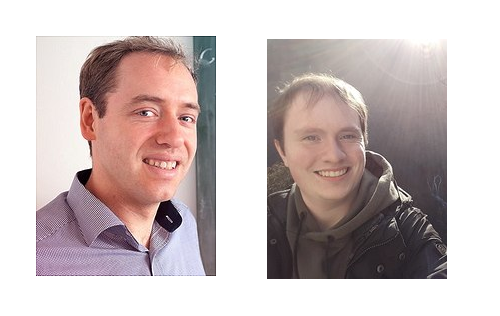
\includegraphics[width=0.8\textwidth]{figs/People Tim.png}
			\end{center}	
		\end{column}
		\begin{column}{0.5\textwidth}

			
			\begin{center}
				Uppsala - Quantum Matter Theory
				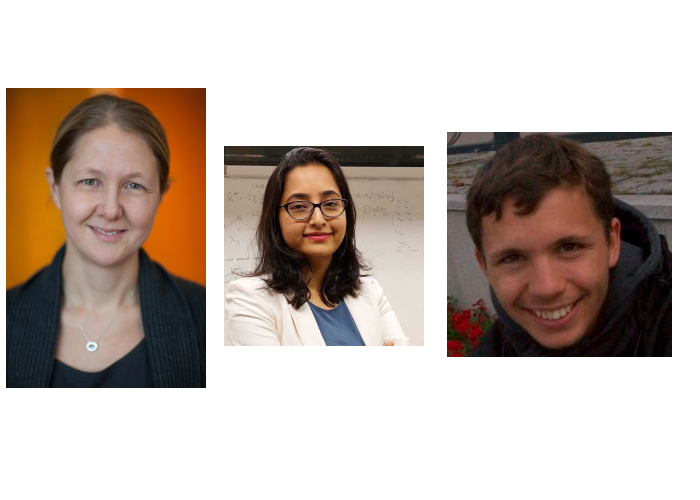
\includegraphics[width=0.9\textwidth]{figs/People Annica.png}
			\end{center}
		\end{column}
	\end{columns}
\end{frame}

\begin{frame}
	From review \cite{tormaSuperconductivitySuperfluidityQuantum2022}
	
	Goal for superconductivity (in terms of technical applications): High transition temperatures
	
	Routes to achieve that:
	\begin{itemize}
		\item Explore classes of materials that show high \(T_C\) (e.g. Cuprates)
		\item More recent: take simpler and more tunable systems following simple theory guidelines based on flat bands and quantum geometry
	\end{itemize}
\end{frame}

\begin{frame}
	%\frametitle{Flat Bands - A Road to High TC Superconductivity?}
	
	In BCS theory for dispersive bands:
	\begin{equation}
		T_C \propto \exp{(- \frac{1}{U n_0 (E_F)})}
	\end{equation}
			
	In flat bands it is predicted (energy dispersion is constant as function of momentum \(\vb{k}\)):
	\begin{equation}
		T_C \propto U
	\end{equation}
	This is due to the high density of states near the Fermi level and vanishing kinetic energy, so that interaction effects dominate
	
	This is true for cases where the interaction is larger than the band width
\end{frame}

\begin{frame}	
	Twisted bilayer materials, in particular twisted bilayer graphene: flat bands can be tuned by changing the twist angle
	
	\begin{figure}
		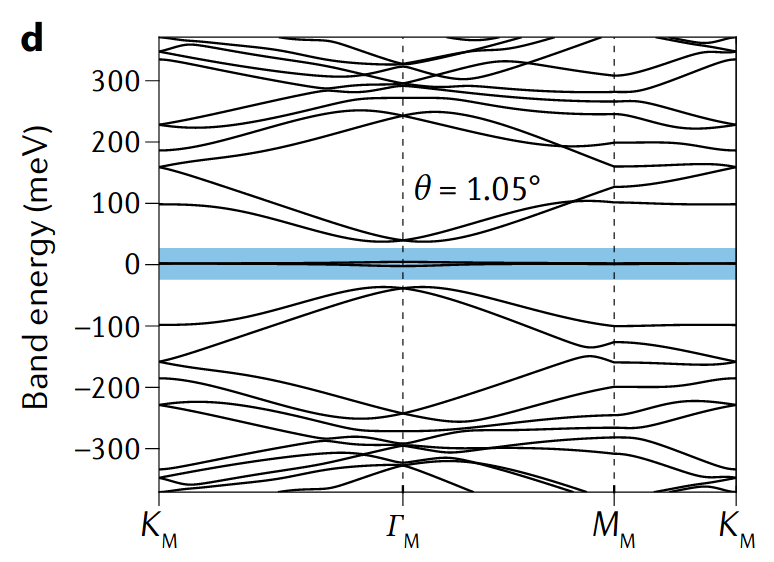
\includegraphics[width=0.3\textwidth]{figs/TBG band structure}
	\end{figure}

	\begin{figure}
		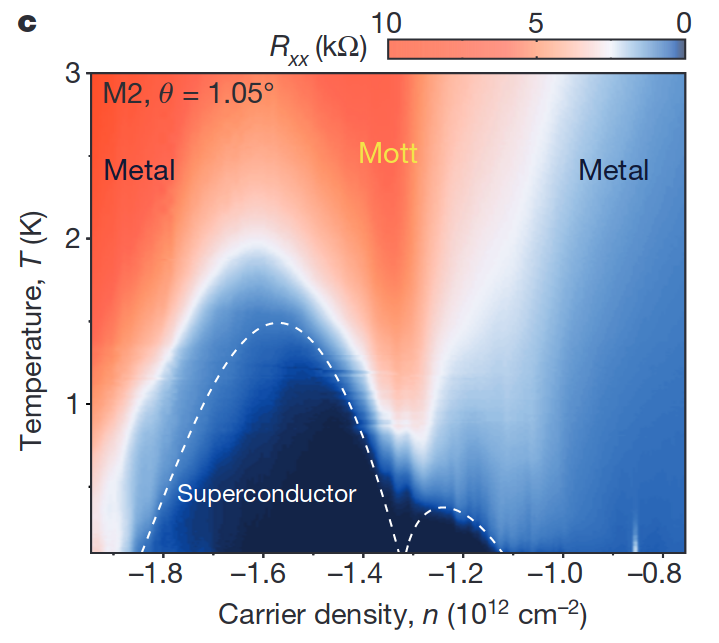
\includegraphics[width=0.3\textwidth]{figs/TBG SC experiment}
	\end{figure}
	
	Experiment: \cite{caoUnconventionalSuperconductivityMagicangle2018}
\end{frame}

\begin{frame}
	%\frametitle{Transport in flat-band systems}
	
	Critical temperature is only one aspect of superconductivity: under this temperature, there is Cooper pairing, but this does not necessarily mean there is a supercurrent
	
	Especially in flat-band systems: group velocity for the non-interacting particles \(v_g = \pdv{\epsilon}{\vb{k}}\), so these dont move
\end{frame}

\begin{frame}
	%\frametitle{Quantum geometry and superfluidity}
	
	Electrodynamic properties of SC materials captured by:
	\begin{equation}
		\vb{j} = -D_S \vb{A}
	\end{equation}
	with current density \(\vb{j}\), vector potential \(\vb{A}\) and superfluid weight \(D_S\)
	
	Describes quantitative description of phenomena of SC (perfect diamagnetism, perfect conductivity), so non-zero superfluid weight is criterion of superconductivity
	
	In single-band BCS theory:
	\begin{equation}
		D_{s, ij} \sim \int \pdv{\epsilon}{k_i,k_j}
	\end{equation}
	Vanishes for a flat band!
	
	
\end{frame}

\begin{frame}
	
	
	Quantum metric determines overlap of Wannier functions, so finite quantum metric means overlap of Wannier functions, so that transport is possible
\end{frame}

\begin{frame}
	%\frametitle{Quantum metric general}
	
	Introduction:
	
	Take Hamiltonian \(\{H(\lambda)\}\) with dependence on some parameters \(\lambda = (\lambda_1, \lambda_2, \ldots)\)
	
	Have eigenenergies \(E_n (\lambda)\) and eigenstates \(\ket{\phi_n (\lambda)}\)
	
	Upon infinitesimally varying \(\odif{\lambda}\), define quantum distance:
	\begin{align}
		\odif{s}^2 &= \vert \vert \psi (\lambda + \odif{\lambda}) \vert \vert^2 = \braket{\fdif{\psi} | \fdif{\psi}} = \braket{\pdif*{\mu} \psi | \pdif*{\nu} \psi} \odif{\lambda^{\mu}} \odif{\lambda^{\nu}} \\
		&= (\gamma_{\mu \nu} + \iu \sigma_{\mu \nu}) \odif{\lambda^{\mu}} \odif{\lambda^{\nu}}
	\end{align}
	To ensure that gauge invariance, add term:
	\begin{equation}
		g_{\mu \nu} (\lambda) \coloneqq \gamma_{\mu \nu} (\lambda) - \beta_{\mu} (\lambda) \beta_{\nu} (\lambda)
	\end{equation}
	with Berry connection \(\beta_{\mu} (\lambda) \iu \braket{\phi(\lambda) | \pdif{\mu} \phi(\lambda)}\)

	For two states \(\lambda_I\) and \(\lambda_F\), quantum distance between them:
	\begin{align}
		\vert \braket{\psi (\lambda_F) | \psi(\lambda_I)} \vert = 1 - \frac{1}{2} \int_{\lambda_I}^{\lambda_F} g_{\mu \nu} (\lambda) \odif{\lambda^{\mu}} \odif{\lambda^{\nu}}
	\end{align}
\end{frame}

\begin{frame}
	Concretely, for example in lattice systems:
	
	Measures distance between close points on the band 
\end{frame}

\begin{frame}
	%\frametitle{My system}
	
	Model:
	\begin{figure}
		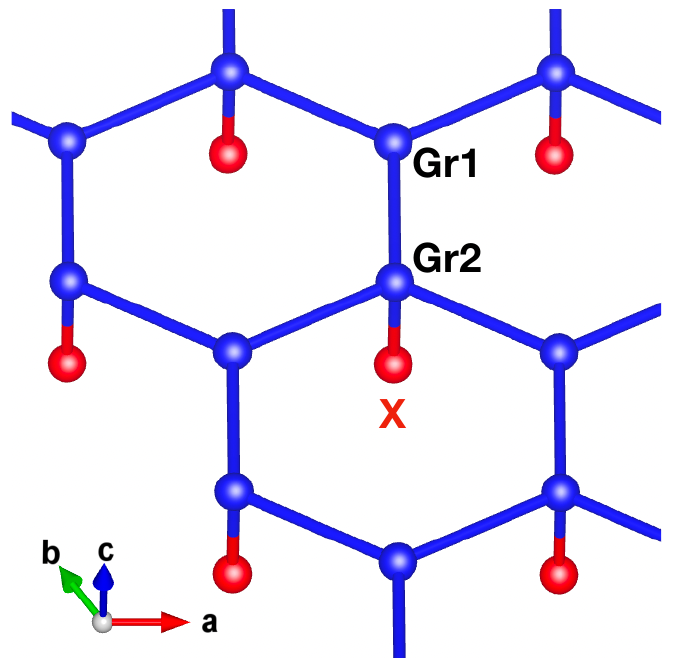
\includegraphics[width=0.3\textwidth]{figs/EG-X structure}
	\end{figure}
	Hexagonal lattice with an additional orbital on one of the sites in the BZ
	
	Non-interacting Hamiltonian:
	\begin{align}
		H_0 &= -t_{\mathrm{X}} \sum_{\langle ij \rangle, \sigma \sigma^{\prime}} d_{i, \sigma}^{\dagger} d_{j, \sigma^{\prime}}
		-t_{\mathrm{Gr}} \sum_{\langle ij \rangle, \sigma \sigma^{\prime}}
		c_{i, \sigma}^{(A), \dagger} c_{j, \sigma^{\prime}}^{(B)} +
		c_{j, \sigma^{\prime}}^{(B), \dagger} c_{i, \sigma}^{(A)} \\
		&+ V \sum_{i, \sigma \sigma^{\prime}} \left(
		d_{i, \sigma}^{\dagger} c_{i, \sigma^{\prime}}^{(A)} +
		c_{i, \sigma}^{(A), \dagger} d_{i, \sigma^{\prime}}
		\right)
		\label{eq:EG-X model Hamiltonian non-interacting}
	\end{align}
	
	Material motivation: Graphene on top of a substrate, different substrates give different values of \(V\)
\end{frame}

\begin{frame}
	
	Band structure:
	
	\begin{figure}
		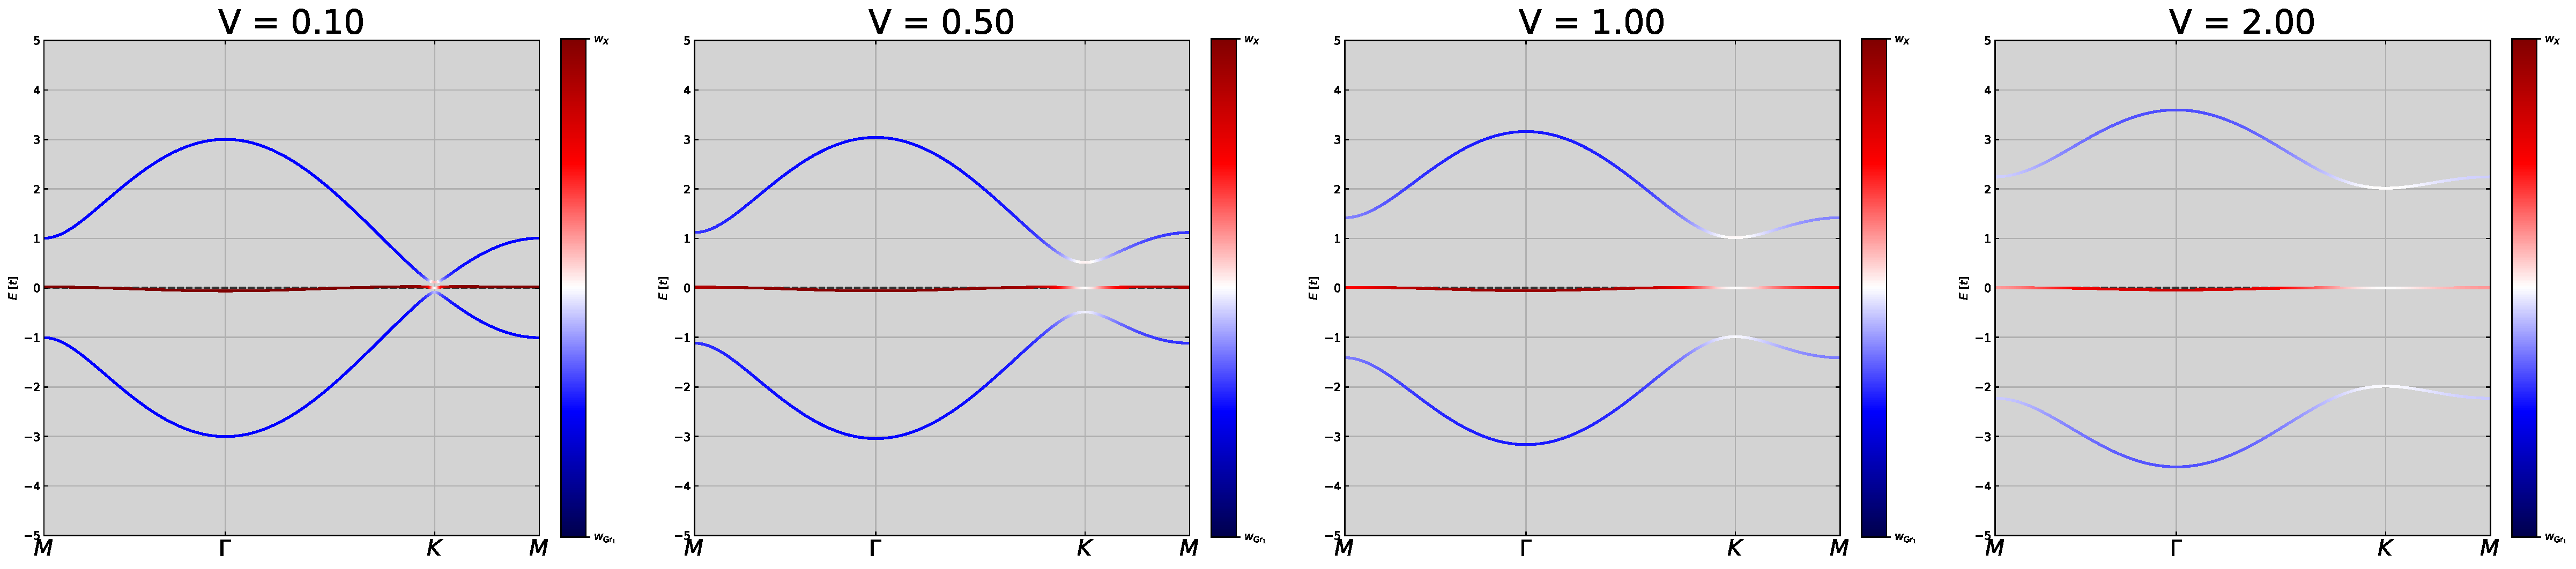
\includegraphics[width=\textwidth]{figs/EG_X bands_tGr_1_tX_0.01}
	\end{figure}

	Important feature:
	\begin{itemize}
		\item Flat band
		\item Hybridization \(V\) determines 
		\item Bands are mixed between the Graphene and X orbitals
	\end{itemize}
\end{frame}

\begin{frame}
	Add local Hubbard interaction:
	\begin{equation}
		H_{\mathrm{int}} = U_{\mathrm{X}} \sum_{i} d_{i, \uparrow}^{\dagger} d_{i, \downarrow}^{\dagger} d_{i, \downarrow} d_{i, \uparrow}
		+ U_{\mathrm{Gr}} \sum_{i, \epsilon=A, B} c_{i, \uparrow}^{(\epsilon) \dagger} c_{i, \downarrow}^{(\epsilon) \dagger} c_{i, \downarrow}^{\epsilon} c_{i, \uparrow}^{\epsilon}
	\end{equation}
\end{frame}
	
\begin{frame}
	\frametitle{Outlook}
	
	Recent preprint by Niklas \cite{wittBypassingLatticeBCSBEC2024}, DMFT calculations on A3C60, getting superfluid weight and coherence length from a finite-momentum constraint on the pairing 
	
	Also recent preprint by Peotta/Törma \cite{penttilaFlatbandRatioQuantum2024} DMFT on Lieb lattice (Flat band system), getting superfluid weight, analysing geometric contribution for finite temperature
\end{frame}


%\begin{frame}
%	\frametitle{Suggestions for Hamburg after 3 months in Sweden}
%\end{frame}


\begin{frame}
	\frametitle{Summary}
	
	\begin{itemize}
		\item Flat bands offer a route
	\end{itemize}

\end{frame}


\end{document}

